\unnumberedChapter{Appendix - Processor Design}

The design of a processor can be approached in many different ways, with choices in instruction set architecture, datapath organization, execution resources, and pipeline structure all influencing the final implementation. The instruction set design is closely connected to the processor design itself, as the operations supported by the architecture determine the required hardware resources and the way instructions are processed.

During the design of the instruction set, the processor model described in this chapter was the envisioned target architecture. The instruction formats, execution model, and available operations were selected with this implementation in mind. Although many different micro architectural implementations are possible, this chapter describes one possible realization of the architecture.

The following sections outline the processor pipeline and describe the purpose of each pipeline stage. Two implementations are presented: a single instruction issue processor, which focuses on simplicity and efficient resource usage, and a dual instruction issue processor, which increases instruction throughput by allowing compatible instructions to execute in parallel.we will sketch a single instruction issue and a dual instruction issue processor.

\unnumberedSection{Pipeline Stages}
%\section*{Pipeline Stages}
%\addcontentsline{toc}{section}{Pipeline Stages}


The reference design implements a three-stage instruction pipeline, with each stage divided into two substages. The pipeline stages and their respective substages are described below. This design allows instruction fetch, decoding, memory access, and execution to overlap, improving overall instruction throughput.

\paragraph{1. Fetch/Decode Stage}
This stage is responsible for retrieving instructions from memory, decoding them, and accessing the register file. It combines the initial instruction fetch with the preparation of operands required for execution.

\subparagraph{Instruction Memory Access Substage}
Fetch the next instruction from the instruction cache using the program state register. The program counter (PC) is updated to point to the next sequential instruction or prepared for a branch target if a branch was predicted in a previous cycle. This substage ensures that the instruction is available for decoding without delay.

\subparagraph{Instruction Decode Substage}
Decode the instruction opcode to determine the operation type, source and destination operands, and any immediate values. This substage also prepares control signals and identifies register file accesses needed for the next stages.

\paragraph{2. Access Stage}
The access stage handles address computation and memory operations. It is responsible for calculating memory addresses for load/store instructions and branch target addresses for conditional or unconditional branches, as well as accessing the data cache when required.

\subparagraph{Address Computation Substage}
Compute memory addresses for load/store instructions or the target address for branch instructions. This includes evaluating effective addresses, offsets, and index computations as required by the instruction.

\subparagraph{Memory Access Substage}
Perform read or write operations to the data cache. This substage ensures that data is available for execution or written back to memory as needed.

\paragraph{3. Execution Stage Substage}
This stage performs arithmetic, logical, and branch resolution operations, committing results to the destination registers or updating the program state register. Both substages are capable of executing a single operation per cycle.

\subparagraph{Execution / Conditional Branch Resolution Substage}
Execute arithmetic or logical instructions and commit the results to the destination registers. For branch instructions, evaluate the branch condition and update the program state register accordingly to reflect the correct next instruction address.


%--------------------------------------------------------------------------------
\unnumberedSection{Single Issue Pipeline}

Twin-64 has a three stage pipeline, with each stage have two subStages. The single issue pipeline processes one instruction at a time through the processor pipeline. Although multiple instructions may be present in different pipeline stages simultaneously, only one instruction is fetched, decoded, and issued during each clock cycle. This organization provides a simple control model while still allowing instruction throughput to approach one instruction per cycle once the pipeline is filled.

The pipeline is divided into three main stages: Fetch/Decode, Access, and Execute. Each stage is further divided into substages to balance the amount of work performed during a clock cycle. The division allows instruction fetch, operand preparation, memory access, and execution of different instructions to overlap.

\begin{figure}[H]
\begin{center}
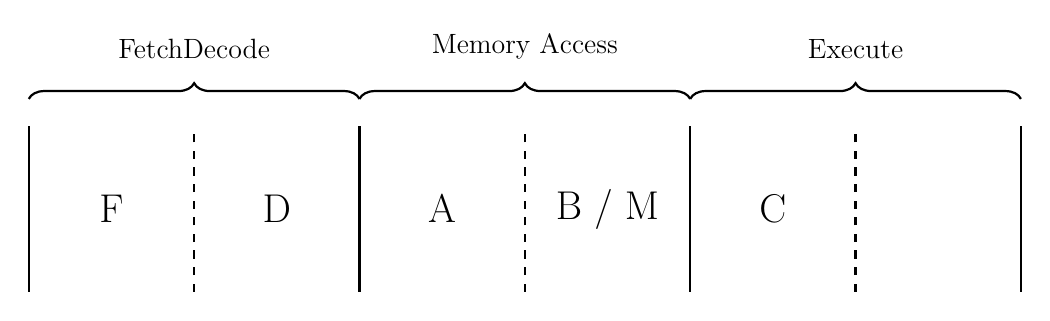
\begin{tikzpicture}[scale=0.7, transform shape]
        
  	%\draw[help lines, gray!70, dashed] (0,0) grid(20,4);
  	
  	\def\height{3}
  	\def\stageWidth{6}
  	\def\subStageWidth{\stageWidth / 2 } 
  	
  	\def\leftOfs{1}
  	\def\fdStageLeftOfs{\leftOfs}
  	\def\maStageLeftOfs{\fdStageLeftOfs+\stageWidth}
  	\def\exStageLeftOfs{\maStageLeftOfs+\stageWidth}
  	
	%separators
	\draw[thick] (\fdStageLeftOfs, 0) -- (\fdStageLeftOfs, \height);
	\draw[thick, dashed] 
		(\fdStageLeftOfs + \subStageWidth, 0) -- 
			(\fdStageLeftOfs + \subStageWidth, \height);
	
	\draw[thick] (\maStageLeftOfs, 0) -- (\maStageLeftOfs, \height);
	\draw[thick, dashed] 
		(\maStageLeftOfs + \subStageWidth, 0) -- 
			(\maStageLeftOfs + \subStageWidth, \height);
	
	\draw[thick] (\exStageLeftOfs, 0) -- (\exStageLeftOfs, \height);
	\draw[thick, dashed] 
		(\exStageLeftOfs + \subStageWidth, 0) -- 
			(\exStageLeftOfs + \subStageWidth, \height);
	
	\draw[thick] (\exStageLeftOfs + \stageWidth, 0) -- 
		(\exStageLeftOfs + \stageWidth, \height);
		
	% brackets
	\draw[thick, decorate, decoration={brace, amplitude=0.2cm}] 
		(\fdStageLeftOfs,\height+0.5) -- (\fdStageLeftOfs + \stageWidth,\height+0.5 )
  		node[midway, yshift=0.6cm, anchor=south] {\Large FetchDecode};
  		
  	\draw[thick, decorate, decoration={brace, amplitude=0.2cm}] (
  		\maStageLeftOfs, \height+0.5) -- (\maStageLeftOfs + \stageWidth, \height+0.5 )
  		node[midway, yshift=0.6cm, anchor=south] {\Large Memory Access};
  		
  	\draw[thick, decorate, decoration={brace, amplitude=0.2cm}] 
  		(\exStageLeftOfs,\height+0.5) -- (\exStageLeftOfs + \stageWidth, \height+0.5 )
  		node[midway, yshift=0.6cm, anchor=south] {\Large Execute};
  		
  	% text
  	\node at ( \fdStageLeftOfs + \subStageWidth / 2, \height / 2 ) {\huge F};
  	\node at (\fdStageLeftOfs + \subStageWidth + \subStageWidth / 2, \height / 2 ) {\huge D};
  	
  	\node at ( \maStageLeftOfs + \subStageWidth / 2, \height / 2 ) {\huge A};
  	\node at (\maStageLeftOfs + \subStageWidth + \subStageWidth / 2, \height / 2 ) {\huge B / M};
    	
  	\node at ( \exStageLeftOfs + \subStageWidth / 2, \height / 2 ) {\huge C};
  
\end{tikzpicture}
\end{center}
\caption{Single Instruction Pipeline}
\label{fig:Single Instruction Pipeline}
\end{figure}

\subparagraph{Fetch/Decode Stage}
The Fetch/Decode stage retrieves the next instruction from the instruction cache and decodes the instruction format. The decoder determines the operation type, identifies the source and destination registers, and prepares any immediate values required by the instruction. Register operands are read during this stage and passed to the following pipeline stages.

\subparagraph{Access Stage}
The Access stage performs address calculation and memory operations. For load and store instructions, the effective memory address is calculated using a dedicated address generation unit. Address calculations use 32-bit adders, which are sufficient for the processor's memory addressing requirements. The data cache is accessed during this stage when required.

\subparagraph{Execute Stage}
The Execute stage performs the actual instruction operation and commits the result. Arithmetic and logical instructions use the 64-bit ALU, while branch instructions are evaluated and resolved during this stage. System instructions perform control register operations or other processor management functions.

Since only one instruction is issued per cycle, all instructions share the same execution resources. This removes the need for complex instruction pairing logic and simplifies hazard detection and pipeline control. The single issue design therefore provides a compact and efficient processor implementation, while the dual issue pipeline extends this foundation by allowing compatible instructions to make use of additional pipeline parallelism.


%--------------------------------------------------------------------------------
\unnumberedSection{Dual Issue Pipeline}

The dual issue pipeline extends the single issue design by allowing two independent instructions to be processed simultaneously. The pipeline stages remain divided into Fetch/Decode, Access, and Execute stages, but the Access and Execute stages contain additional resources to allow two compatible instructions to proceed in parallel.

The instruction decoder identifies two instructions that can be paired and determines whether their resource requirements are compatible. The processor supports parallel execution of different instruction classes, including Compute, Branch, Memory, and System instructions. The following instruction combinations are supported:

\begin{center}
\begin{tabular}{c|l}
\textbf{Combination} & \textbf{Description} \\
\hline
CC & Two Compute instructions executed in parallel \\
CM & Compute instruction paired with a Memory instruction \\
CB & Compute instruction paired with a Branch instruction \\
CS & Compute instruction paired with a System instruction \\
BM & Branch instruction paired with a Memory instruction
\end{tabular}
\end{center}

Other combinations are not issued together and are executed as separate instructions. This restriction simplifies hazard detection, resource allocation, and pipeline control while still allowing the most common instruction sequences to benefit from dual issue execution.

\begin{figure}[H]
\begin{center}
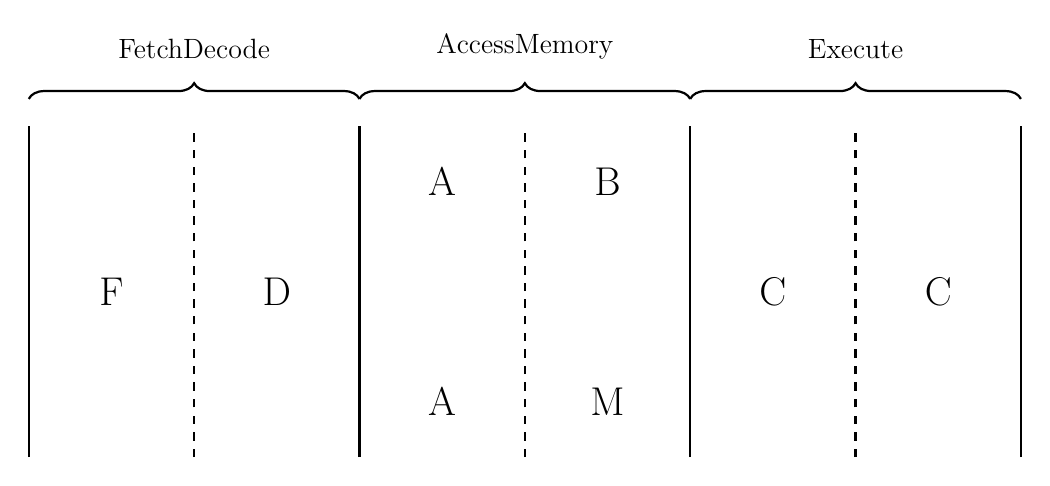
\begin{tikzpicture}[scale=0.7, transform shape]
        
  	%\draw[help lines, gray!70, dashed] (0,0) grid(20,8);
  	
  	\def\height{6}
  	\def\stageWidth{6}
  	\def\subStageWidth{\stageWidth / 2 } 
  	
  	\def\leftOfs{1}
  	\def\fdStageLeftOfs{\leftOfs}
  	\def\maStageLeftOfs{\fdStageLeftOfs+\stageWidth}
  	\def\exStageLeftOfs{\maStageLeftOfs+\stageWidth}
  	
  	
	%separators

	\draw[thick] (\fdStageLeftOfs, 0) -- (\fdStageLeftOfs, \height);
	\draw[thick, dashed] 
		(\fdStageLeftOfs + \subStageWidth, 0) -- 
			(\fdStageLeftOfs + \subStageWidth, \height);
	
	\draw[thick] (\maStageLeftOfs, 0) -- (\maStageLeftOfs, \height);
	\draw[thick, dashed] 
		(\maStageLeftOfs + \subStageWidth, 0) -- 
			(\maStageLeftOfs + \subStageWidth, \height);
	
	\draw[thick] (\exStageLeftOfs, 0) -- (\exStageLeftOfs, \height);
	\draw[thick, dashed] 
		(\exStageLeftOfs + \subStageWidth, 0) -- 
			(\exStageLeftOfs + \subStageWidth, \height);
	
	\draw[thick] (\exStageLeftOfs + \stageWidth, 0) -- 
		(\exStageLeftOfs + \stageWidth, \height);
		
	% brackets
	\draw[thick, decorate, decoration={brace, amplitude=0.2cm}] 
		(\fdStageLeftOfs,\height+0.5) -- (\fdStageLeftOfs + \stageWidth,\height+0.5 )
  		node[midway, yshift=0.6cm, anchor=south] {\Large FetchDecode};
  		
  	\draw[thick, decorate, decoration={brace, amplitude=0.2cm}] (
  		\maStageLeftOfs, \height+0.5) -- (\maStageLeftOfs + \stageWidth, \height+0.5 )
  		node[midway, yshift=0.6cm, anchor=south] {\Large AccessMemory};
  		
  	\draw[thick, decorate, decoration={brace, amplitude=0.2cm}] 
  		(\exStageLeftOfs,\height+0.5) -- (\exStageLeftOfs + \stageWidth, \height+0.5 )
  		node[midway, yshift=0.6cm, anchor=south] {\Large Execute};
  		
  	% text
  	\node at ( \fdStageLeftOfs + \subStageWidth / 2, \height / 2 ) {\huge F};
  	\node at (\fdStageLeftOfs + \subStageWidth + \subStageWidth / 2, \height / 2 ) {\huge D};
  	
  	\node at ( \maStageLeftOfs + \subStageWidth / 2, \height - 1 ) {\huge A};
  	\node at (\maStageLeftOfs + \subStageWidth + \subStageWidth / 2, \height - 1 ) {\huge B};
  	
  	\node at ( \maStageLeftOfs + \subStageWidth / 2, 1 ) {\huge A};
  	\node at (\maStageLeftOfs + \subStageWidth + \subStageWidth / 2, 1 ) {\huge M};
  	
  	\node at ( \exStageLeftOfs + \subStageWidth / 2, \height / 2 ) {\huge C};
  	\node at (\exStageLeftOfs + \subStageWidth + \subStageWidth / 2, \height / 2 ) {\huge C };

	
\end{tikzpicture}
\end{center}
\caption{Dual Instruction Pipeline}
\label{fig:DUal Instruction Pipeline}
\end{figure}


\subparagraph{Fetch/Decode Stage}
The Fetch/Decode stage retrieves up to two instructions from the instruction cache and decodes their operation type and operand requirements. The decoder determines whether the instructions form a valid pair and generates the required control signals for the following stages. Register operands are read during this stage, allowing both instructions to enter the pipeline with their operands already available.

\subparagraph{Access Stage}
The Access stage performs address generation and memory operations. Memory address calculation uses dedicated 32-bit adders, as the address space requirements do not require the full 64-bit arithmetic datapath. A Memory instruction can therefore calculate its effective address while another instruction performs an independent operation.

For load and store instructions, the memory access substage communicates with the data cache. The pipeline supports pairing a Memory instruction with a Compute or Branch instruction, provided that no data dependency or resource conflict exists.

\subparagraph{Execute Stage}
The Execute stage performs arithmetic, logical, branch resolution, and system operations. The processor contains a single 64-bit ALU. This is sufficient because the two execution substages are separated in the pipeline and each substage can produce one result per cycle. A dual issue cycle therefore does not require two independent ALUs; instead, the existing execution resource is reused across the pipeline stages.

Compute instructions use the 64-bit ALU for arithmetic and logical operations, while Branch instructions use the execution stage for condition evaluation and program state updates. System instructions use the execution resources for control register access and privileged processor operations.

The dual issue pipeline improves instruction throughput by allowing independent instructions to overlap while avoiding unnecessary duplication of expensive execution resources. The supported instruction pairing rules provide a balance between increased performance and hardware complexity.

%--------------------------------------------------------------------------------
\unnumberedSection{Design Rationale}

The Twin-64 architecture follows the principle of keeping the hardware implementation simple while allowing the compiler to assist in exposing instruction-level parallelism. Instead of relying on complex dynamic scheduling mechanisms to discover parallel execution opportunities at runtime, the processor defines a small number of well-known instruction combinations that can execute together.

By limiting the scope of dual issue execution, the hardware required for instruction decoding, dependency checking, and resource allocation remains manageable. The compiler can take advantage of the available parallelism by scheduling compatible instructions, while the processor only needs to verify that the selected instruction pair can safely execute.

This approach provides improved instruction throughput without introducing the hardware complexity associated with wide superscalar or out-of-order processors. The design represents a balance between implementation simplicity and execution efficiency: the processor provides the capability for parallel execution, while the compiler remains responsible for making effective use of that capability.

The name Twin-64 reflects this design choice. The architecture combines a 64-bit processor model with two cooperating instruction paths, allowing two compatible instructions to progress through the pipeline together while maintaining a simple and predictable hardware design.

 
